\chapter{Experimental setup} \label{experiment}

\begin{itemize}
\item description of MAMI, how the beam is produced, how the electrons are polarized.
\item description of A1.
\item description of beam stabilization, how the monitors measure the beam parameters.
\item Electronics description, DAQ system, VFC monitors.
\item Detectors A and B.
\end{itemize}

\section{First description of the experiment}

First description of the experiment, how we want to collect data, new picture of the kinematic of the experiment. Maybe here it's a good point to describe the structure of the event.

\section{Mami}
How Mami produces polarized electron and how the particle are accelerated (the way Mainz Mikroton is working is completely different from the other accelerators, so maybe this section will be too long).

\subsection{Acceleration stage}
explain how electrons are accelerated, and sent to different experiments.


\subsection{Polarized Beam}
%Here a subsection to explain how the polarized electrons are produced. Important to mention the systematic error for the polarization mesurement (in our beam time we couldn't measure with Moller polarimeter, so this discussion is important for future experiment, however it's important to say something about it). Remember to explain how the spin are rotated to the transverse plane, and the $\frac{\lambda}{2}$

For the beam-normal single spin asymmetry a vertical polarized beam is necessary. At the MAMI electron accelerator is possible to produce a vertical polarized beam with energy in the range $\SI{180}{\mega \electronvolt} - \SI{855}{\mega \electronvolt}$. In this section the procedure to orient the beam vertically, following an explanation of how the degree of polarizarion of the beam is measured.

The electron source used at MAMI is made by a strained GaAs/GaAsP superlattice photocathode 
illuminated by circular polarized light. A Pockels cell changes the helicity of the photons impinging on the electrons. The extracted electron has the same helicity of the incoming photon, let's suppose as an example:

\begin{center}
\begin{equation}
\feynmandiagram [scale = 0.8, transform shape][baseline = (g)]{
	a [particle = \(e^{-}\)] -- [fermion] b  -- [fermion] c [particle = \(e^{-}\)],
	b -- [boson] d [particle = \(\gamma\)],};
\hspace{2cm}
(Jz)_{\gamma} = \pm 1 \qquad (Jz)_{e^{-}} = \mp \frac{1}{2} \rightarrow \pm \frac{1}{2}
\end{equation}
\end{center}

With the fast change of the Pockels cell it is possible to alternately revert the sign of the polaritazion. By the insertion of a $\lambda/2$ plate between the laser system and the photochatode the polarization orientation of the electron beam can be reversed for each sub-event, useful later for the estimation of systematic errors.

To switch from longitudinal polarization to transverse polarisation, two devices are used: the \textbf{Wien filter} and a \textbf{double solenoid} located in the injection beam line. 

\begin{figure}[hbtp]
\centering
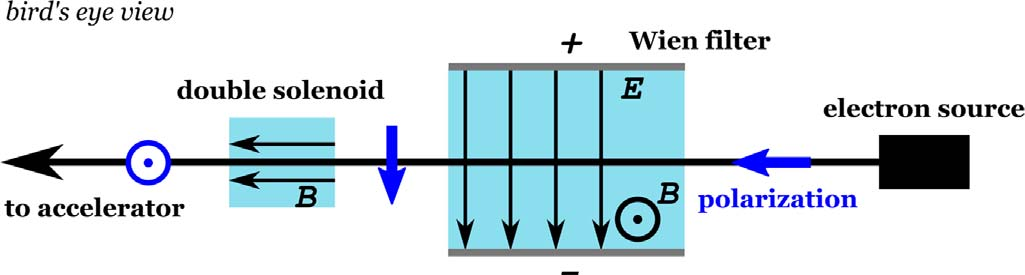
\includegraphics[width = \textwidth]{ExperimentalSetup/injection.png}
\caption{Setup for the trasverse polarization.}
\end{figure}

Following the picture, the longitudinal polarized electron from the source are rotated first in the XY plane, to obtain the trasverse polarization, then with subsequent double solenoid the spins are rotate in the vertival direction. 
After this allignement the electrons go through the accelerator to the experimental hall. The spins then precesses during this time in the magnetic fields of the accelerator's bending magnets, following the BMT equation.
In our experiment, because of the vertical polarization, only the residual horizontal component precedes during the motion. For conventional experiment the polarization vector is rotated by the Wien filter with an angle such that the polarization si longitudinally aligned in the experimental hall, considering that after the rotation, the polarization is affected by another rotation due to the spin precession. The rotation angles of the polarization vector through the accelerator are known from simulations and are also directly measured for relevant energies, for a beam of $\SI{570}{\mega \electronvolt}$ the rotation angle is $\ang{55}$ with an accuracy of $\pm \ang{2}$
At the beginning MAMI was not developed with the aim a trasverse beam. So it's not possible to measure directly the polarization for the vertical axis. However it's possible, with the existing setup, to exstimate the degree of polarization. For this purpose a Moller, Comport and Mott polarimeters are used. The vertical polarization alignment can be accomplished by the minimization of the horizontal components. 

%aggiungere ai riferimenti l'articolo: Vertical Beam Polarization at MAMI. 

\subsection{Mott, Compton and Moller polarimenters}
%Briefly explain how the Mott polarimeter works, for measuring the polarization of the beam.

To Measure the polarization of an electron beam different polarimeters can be used. Here we explain briefly the physics underlying the \textit{Mott} polarimeter, used in the experiment.
Consider an electron beam that is sent towards a nucleus of charge $Ze$. We know from theory that the spin of the incident electron is affected by the electromagnetic field produced by the nucleus. This can be described as:



\begin{align*}
\vec{B}_{nucleus} = \frac{-1}{c} \vec{v} \times \vec{E}_{nucleus} = \frac{Ze}{mc r^{3}} \vec{L} \\
V = - \mu \cdot B_{nucleus} = \frac{Ze}{mcr^{3}} \vec{L} \cdot \vec{S}_{e^{-}}
\end{align*}

We can recognize the spin-orbit interaction here. This term yields the polarization dependence of the cross section. The cross section can be model in the following way

\begin{align*}
\sigma(\theta) = I(\theta) [1 + S(\theta) \vec{P} \cdot ]
\end{align*}

The total beam polarization is measured by a Moller polarimeter, in the experimental hall, with the beam polarization oriented longitudinally in the experimental hall. The Moller polarimeter can measure the longitudinal polarization of the beam.The other two polarimeters, Compton and Mott, located behind the injector linear accelerator (ILAC), are sensitive to the longitudinal and the trasverse horizontal components of the beam (with an energy around $\SI{3.5}{\mega \electronvolt}$ at this stage). The procedure for the allignment is the following: at the beginning of the beam time the Mott polarimeter is used for different settings of the solenoidal field, with the Wien filter angle equal (nominal) to $\ang{90}$. The aim is to minimize the horizonal polarization component after the rotation performed by the double solenoid, changing the solenoidal magnetic field. Then a second optimization follows, using the Moller polarimeter for different Wien filter angles is performed. With the new Wien filter settings, another measurement is performed with the Mott polarimeter.

\section{A1 spectrometers hall}

Describing the A1 room, how the spectrometers are operating (+ figures), a picture of the target and the important parameters, like thickness. Also mention the convention to use target with$10 \%$ of the radiation lenght, to avoid double scattering.  Mention that we need the Wobbler magnet to change the hitting position of the beam to prevent the target from melting.
Then add a picture of the beam-line.

\section{Detectors and beam monitors}

\subsection{Detectors A and B}
Describe the two detectors we placed inside the spectrometers, the $Q^{2}$ for our mesurement. The way the counts are collected, so the expected signal for the Čerenkov detector. Explain also how we will use the old detectors of the two spektrometers to align the elastic scattering plane to our detectors.

\subsection{Monitors and stabilization}
Explain how the monitors for the beam parameters work. (this section could be long, however the way these parameters are measured is particular, so it's important to explain everything properly).

\section{Electronics}
Short introduction about the old electronics setup and why a new versions is needed, then describe all the electronics used for our experiment:
\begin{itemize}
\item Nino board for collecting the data from the pmts
\item VFCs for collecting the data from X21,X25,Y21,Y25,ENMO,I21,I13
\item master board for collecting the monitors data/controlling the source/wobbler magnets.
\item small boxes for switching from new electronic read-out to the old electronics read-out (spectrometers DAQ)
\end{itemize}

